\section{実験原理}
\subsection{電離平衡}
酸HAは(\ref{equ:heiko})式のように電離し,平衡に達する.また電離定数(または酸解離定数)$K_A$を(\ref{equ:teisu})式で定義する.
また$K_A$を用いて$pK_A$を(\ref{equ:pka})式で定義する.
\begin{equation}
  \label{equ:heiko}
  HA\rightleftharpoons H^+ + A^-
\end{equation}
\begin{equation}
  \label{equ:teisu}
  K_A=\cfrac{[H^+][A^-]}{[HA]}
\end{equation}
\begin{align}
  \label{equ:pka}
  \begin{aligned}
    pK_A&=-\log K_A\\
    &=pH-\log \cfrac{[A^-]}{[HA]}
  \end{aligned}
\end{align}
半中和点において$\cfrac{[A^-]}{[HA]}=1$であり,\ $pK_A=pH$が成り立つ.故に半中和点での$pH$を測定することで
電離定数$K_A$を算出できる.半中和点は滴定曲線,または示差曲線から求める.(1)滴定曲線を用いる場合,
曲線に傾き$\cfrac{\pi}{4}$の接線を2本引き,これと等距離な曲線上の点を終点とする.
(2)滴定曲線がなだらかな場合,示差曲線のピークを半中和点とすることでより正確に終点を求められる.
これらの方法で求めた終点の横座標が中和当量$v_e$であり,横座標$\cfrac{v_e}{2}$での$pH$が$pK_A$と一致し,これを用いて$K_A$を算出する.
\begin{figure}[htbp]
 \begin{minipage}{0.5\hsize}
  \begin{center}
   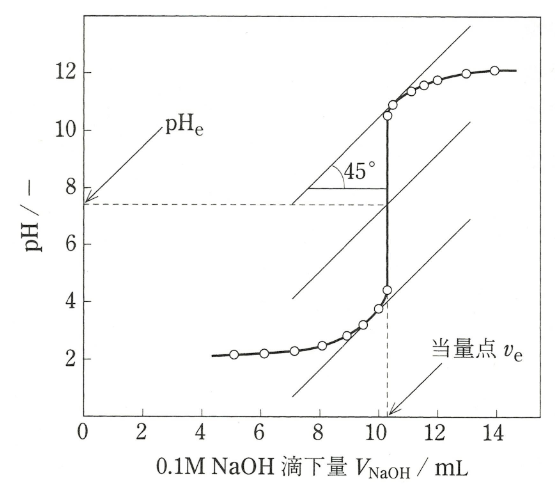
\includegraphics[height=40mm]{tekitei.png}
  \end{center}
  \caption{滴定曲線の例}
 \end{minipage}
 \begin{minipage}{0.5\hsize}
  \begin{center}
   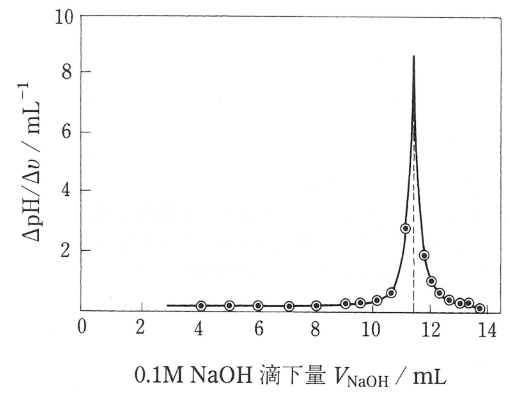
\includegraphics[height=40mm]{sisa.png}
  \end{center}
  \caption{示差曲線の例}
 \end{minipage}
\end{figure}
%\subsection{ファクター$f$}
%調製した際の名目濃度$C$には誤差があるため,標準溶液で標定して得た真の濃度$C'$との補正係数として
%ファクター$f$を用いる.これらの間には以下の関係が成り立つ.
%\begin{equation}
%  \label{equ:factor}
%  C'=Cf
%\end{equation}
%\newpage
